\section{Laden und Übersetzen der Hard- und Software} \label{sec: laden_und_uebersetzen}

Bevor eine Online-Verbindung mit der SPS aufgebaut werden kann, wird die Hard- und Software übersetzt (\autoref{fig:Bild6.1}) und anschließend in das Gerät geladen (\autoref{fig:Bild6.2}).

\begin{figure}[H]
   \centering
   \fbox{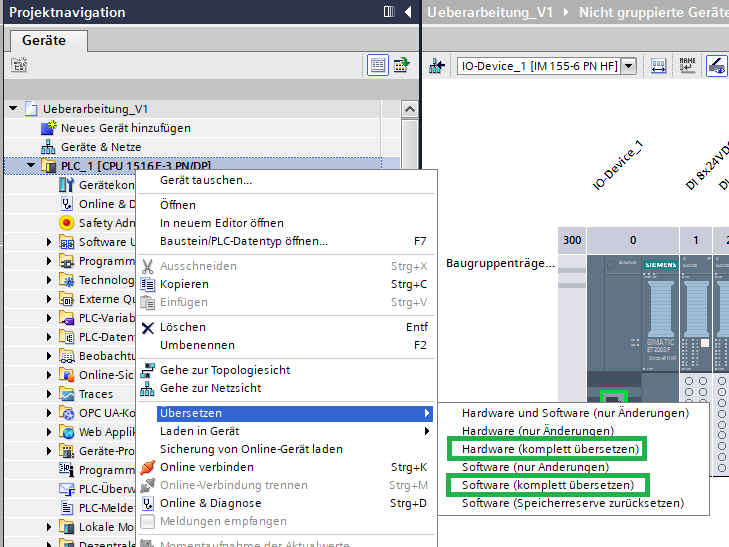
\includegraphics[width=0.6\textwidth]{Bilder/6. Laden und Übersetzen der Hard- und Software/(6.1) Uebersetzen.PNG}}
   \caption[Übersetzen der Hard- und Software]{Übersetzen der Hard- und Software}
   \label{fig:Bild6.1}
\end{figure}

\begin{figure}[H]
   \centering
   \fbox{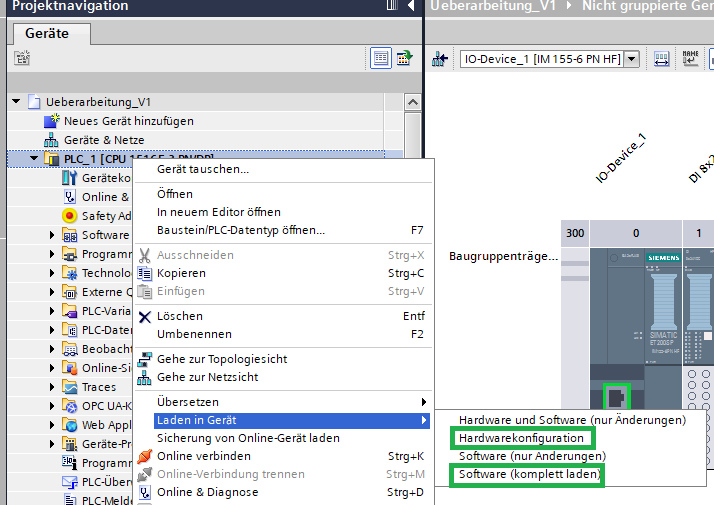
\includegraphics[width=0.6\textwidth]{Bilder/6. Laden und Übersetzen der Hard- und Software/(6.2) Laden.PNG}}
   \caption[Laden der Hard- und Software]{Laden der Hard- und Software}
   \label{fig:Bild6.2}
\end{figure}